\chapter{Requirement and Analysis}
\section{Introduction}
The overall purposes of this study is to improve efficiencies of \gls{ic}'s digital document management strategies. 
The study involves investigating internal \gls{ic}'s working procedures and regulations, how \gls{ic} execute strategies on their digital document assets; what are advantages and disadvantages of their strategies.
Gaining such information is valuable to this study because plausible solutions could be proposed and implemented. 
Solutions that could further improve flows of documents inside \gls{ic}.
This chapter presents requirement gathering methods to address the problem.

\section{Gathering Requirements}
Section \ref{sec:motivation} introduces digital document problems occurred inside \gls{ic}.
These problems were formulated to research questions suitable for this study.
The study's goal is to create a system to verify the hypotheses posed by two research questions:
\begin{enumerate}
	\item How to store and retrieve digital \gls{ic}'s documents so that authorized users can access within \gls{ic}, \gls{kmitl} precinct?
	\item How to track \gls{ic}'s document going through each task specified by \gls{ic}'s document workflow?
\end{enumerate}
This study implements qualitative research method with two research strategies: interview and case study.
The following sections discuss these two strategies in more detail.

\subsection{Interview}
\citeauthor{gall7j} (\citeyear{gall7j}) states that interview is the spontaneous generation of questions in a natural interaction, typically one that occurs as part of ongoing participant observation fieldwork.
\citeauthor{brady2011craft} (\citeyear{brady2011craft}) points out that what interviewer and salesman have in common is potential customers whom one could hold their attention to talk.
Getting an interview means making an appointment to see the subject, identifying questions related to the research topic, and showing on time for the interview.
The purpose of interview is to gain information from interviewee by having interviewer asking questions.
Researchers can gain useful insights from the subject who is expertise in one's field.

Figure \ref{ic-org-sturcture} shows \gls{ic}'s organization structure.
The top-most is the dean followed by deputy dean then assistant of deputy dean.
On the right hand side are committee members.
Only academic and academic support located at the bottom-most hierarchy involves archiving documents.
 \begin{figure}[h]
 	\centering
 	\caption{\gls{ic} organization's structure}
 	\label{ic-org-sturcture}
 	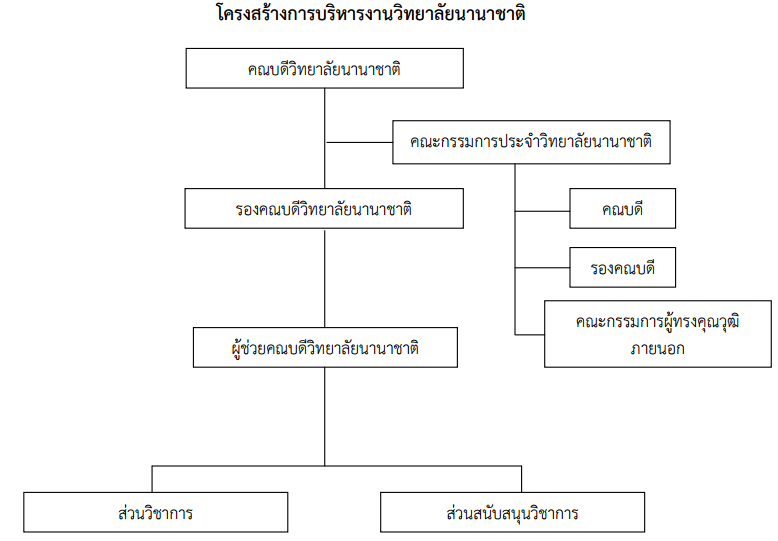
\includegraphics[scale=0.7]{res/Methodology/ic-org}
 \end{figure}

In this study, \gls{ic} staffs are the subject of this study divided into two focus groups:
\begin{description}
	\item [Academic staffs (the bottom-most hierarchy)] as a primary focus group because they are responsible for keeping records of all \gls{ic}'s documents.
	Transfer documents around the organization according to \gls{ic}'s workflow specifications.
	Managing day-to-day operations within the organization.
	They also provide academic advices and guidances to \gls{ic} undergraduate and postgraduate students.

	\item [Administrative staffs] as a secondary focus group because they are directly involve in keeping and organizing documents.
	Some of them have privilege to issue, review, and approve documents.
	In order to know more about their procedures, deputy dean and deputy dean's assistant are selected as a sample for this study.
\end{description}

After conducted an interview, \gls{ic} staffs reveal that they would like a system that manage their organization's documents automatically.
What they mean by managing is that they would like to know what are they suppose to do with received documents.
Things they have to do could be approval, signing, or printing documents.
Then, forwarding the document to another person in organization without necessarily having to know who that person is.
They also would like to know any additional documents required before forwarding documents so that they can prepare them beforehand.

For every official \gls{ic}'s documents, \gls{ic} assigns an identification number internally.
There are 11 types of documents separated into three categories based on head of the department who is responsible for those documents as shown in table \ref{tbl-doc-subtype}.
\begin{table}[h]
	\caption{Document type with identification code separated by category}
	\label{tbl-doc-subtype}
	\centering
\begin{tabular}{llC{3cm}}
	\hline
	Category & Document Type & Identification Code \\
	\hline
	General Management 1 & Archive & AA \\
	General Management 1 & Human Resources & AB \\
	General Management 1 & Quality Assurance & AC \\
	General Management 1 & Parcel & AD \\
	General Management 1 & IT/KM & AE \\
	\midrule
	General Management 2 & Plan and Risk Management & BA \\
	General Management 2 & Accounting & BB \\
	General Management 2 & Research & BC \\
	General Management 2 & Academic Management & BD \\
	\midrule
	Academic & Academic Administration & CA \\
	Academic & Student Affairs & CB \\
	\hline
\end{tabular}
\end{table}

According to the scope stated in Section \ref{sec:scope}, each documents is associated with the document as shown in table \ref{tbl-scope-doc-subtype}.
External documents are not \gls{ic}'s official documents in table \ref{tbl-doc-subtype}.
They are attachments of the official document.
\begin{table}
	\centering
	\caption{Association between document stated in \ref{sec:scope} and document type in table \ref{tbl-doc-subtype}}
	\label{tbl-scope-doc-subtype}
\begin{tabular}{ll}
	Document Form & Document Type \\
	\hline
	Absence Form & Academic Administration \\
	Student Internship Form & Student Affairs \\
	Conference Outside \gls{kmitl} Form & Academic Administration \\
	\hline
\end{tabular}
\end{table}

To generate an identification number for a document, it has to confine to the following format: $TTYYYYDDDD$.
Where $TT$ is the identification code from table \ref{tbl-doc-subtype}.
$YYYY$ is the four-digit full Christian year such as 2016 or 2015.
$DDDD$ is the four-digit number of the document.
It starts at one and must increment by one each time as the new document is created.
If $DDDD$ is less than one thousand, it must fill with leading zeros until there are four digits presents.
If the number is greater than 9999 which is a maximum limit, it has to continue counting normally but without- any leading zeros.
Although, having the same type of document more than ten thousand documents has never happened to \gls{ic} before.
If new year has started, the $DDDD$ must reset back to one (0001).

To clarify how the identification number is generated and combined together, let's assumes that \gls{ic} already have two documents of type \enquote{Academic Administration}.
Mr. X would like to take a vacation on May, 2016.
So he requests an \enquote{Absence Form} and put in an information.
Then, he submits the form to the system.
The absence form is a part of academic administration so $TT$ is \enquote{CA}.
The document is created at 2016 so $YYYY$ is \enquote{2016}.
Because there are two documents already in the system.
The next number is three so $DDDD$ is \enquote{0003}.
Combining $TT$, $YYYY$, and $DDDD$ together yields CA20160003.

\subsection{Case Study}
\citeauthor{merriam1988case} (\citeyear{merriam1988case}) defines case study as an intensive study of a single unit for the purpose of understanding a larger class of similar units.
Unit refers to an observed sample at a discrete point in time.
Each unit comprises of cases built from variables upon observations.
For example, an analysis of worldwide smartphone sales in fourth quarter of 2011 \cite{goasduff2012gartner}.
Samples are mobile devices.
Units are worldwide mobile sales to end users observed in fourth quarter of 2010 and 2011.
Cases are sales by vendor and sales by operating system.
Variables are total number of sales (thousands of units) and market share percentage.
Figure \ref{tbl:ex-case-study-var} shows \citeauthor{goasduff2012gartner}'s case study \cite{goasduff2012gartner} in hierarchy based on \citeauthor{merriam1988case}'s definition.
A unit (sales in fourth quarter) are constructed from two sub units based on years---2010 and 2011.
Sub units in figure \ref{tbl:ex-case-study-var} are split to another column to preserve space.

\begin{figure}[h]
	\caption{Samples, units, cases, and variables for \citeauthor{goasduff2012gartner}'s case study \cite{goasduff2012gartner}}
	\label{tbl:ex-case-study-var}
\begin{tabular}{ll}
	\begin{minipage}{8cm}\dirtree{%
		.1 Mobile Devices.
			.2 Sales in Fourth Quarter.	
				.3 2010.
					.4 By Vendor.
						.5 Total Sales (Thousands of Units).
						.5 Market Share (\%).
					.4 By Operating System.
						.5 Total Sales (Thousands of Units).
						.5 Market Share (\%).
		}
	\end{minipage}
	&
	\begin{minipage}{8cm}\dirtree{%
		.1 Mobile Devices.
			.2 Sales in Fourth Quarter.	
				.3 2011.
					.4 By Vendor.
						.5 Total Sales (Thousands of Units).
						.5 Market Share (\%).
					.4 By Operating System.
						.5 Total Sales (Thousands of Units).
						.5 Market Share (\%).
		}
	\end{minipage}
\end{tabular}
\end{figure}

Conducting case studies based on \citeauthor{merriam1988case}'s definition can yield concrete results.
\citeauthor{merriam1988case}'s definition offers an advantage to study the same case in different point of time.
It also allows variables to be unquantifiable as \citeauthor{merriam1988case} states that variables are built from observation.

This study utilizes \citeauthor{merriam1988case}'s case study model to construct case studies as shown in figure \ref{fig:our-case-study-method}.
Documents are a sample.
\gls{ic}'s documents observed in 2015 is a unit.
There are three cases;
\begin{enumerate*}
	\item storing digital documents;
	\item retrieving digital documents;
	\item tracking digital documents.
\end{enumerate*}
First and second unit comes from the second research question.
Thrid unit comes from the third research question.
Each case comprises of four variables;
\begin{enumerate*}
	\item absence form;
	\item student internship form;
	\item conference outside \gls{kmitl} form;
	\item external document.
\end{enumerate*}
They come from the scope stated in section \ref{sec:scope}.

\begin{figure}[h!]
	\centering
	\caption{Samples, units, cases, and variables for case study of this research}
	\label{fig:our-case-study-method}
	\begin{minipage}{8cm}\dirtree{%
		.1 Documents.
		.2 \gls{ic}'s Documents Observed in 2015.
		.3 Storing Digital Documents.
		.4 Absence Form.
		.4 Student Internship Form.
		.4 Conference Outside \gls{kmitl} Form.
		.4 External Digital Documents.
		.3 Retrieving Digital Documents.
		.4 Absence Form.
		.4 Student Internship Form.
		.4 Conference Outside \gls{kmitl} Form.
		.4 External Digital Documents.
		.3 Tracking Digital Documents.
		.4 Absence Form.
		.4 Student Internship Form.
		.4 Conference Outside \gls{kmitl} Form.
		.4 External Digital Documents.
		}
	\end{minipage}
\end{figure}

These mentioned forms emerge from a specific type of \gls{ic}'s official documents.
External digital documents are unofficial documents because \gls{ic} isn't the one who issue the documents.
Thus, figure \ref{fig:our-case-study-method} can be rewritten for simplicity as shown in figure \ref{fig:our-case-study-method-rewrite}.
\begin{figure}[h!]
	\centering
	\caption{Simpler version of figure \ref{fig:our-case-study-method}}
	\label{fig:our-case-study-method-rewrite}
	\begin{minipage}{8cm}\dirtree{%
			.1 Documents.
			.2 \gls{ic}'s Documents Observed in 2015.
			.3 Storing Digital Documents.
			.4 Official Documents.
			.4 Unofficial Documents.
			.3 Retrieving Digital Documents.
			.4 Official Documents.
			.4 Unofficial Documents.
			.3 Tracking Digital Documents.
			.4 Official Documents.
			.4 Unofficial Documents.
		}
	\end{minipage}
\end{figure}

The workflow of each type of forms are represented as an activity digram shown in figure \ref{fig:diagram-absence}, \ref{fig:diagram-student-internship}, and \ref{fig:diagram-conference}.
The common operation that appears on all diagram is that someone has to either approve or reject the document.
User is the person who initiate the document, filling forms, and submit to the staff for approval.
\enquote{Absence form} and \enquote{Conference outside \gls{kmitl} form} requires user, staff, and dean to sign the document.
If someone reject the document, user has to be notified about the rejection.
The final process is to \enquote{finalize document} as shown in figure \ref{fig:diagram-finalize-document}.
Staff has to upload attachments as an evidence acquired from scanning to the system. 
Then, the system will notify user that the submitted document has completed successfully.
\begin{figure}[h]
	\centering
	\caption{An activity diagram for \enquote{Absence form}}
	\label{fig:diagram-absence}
	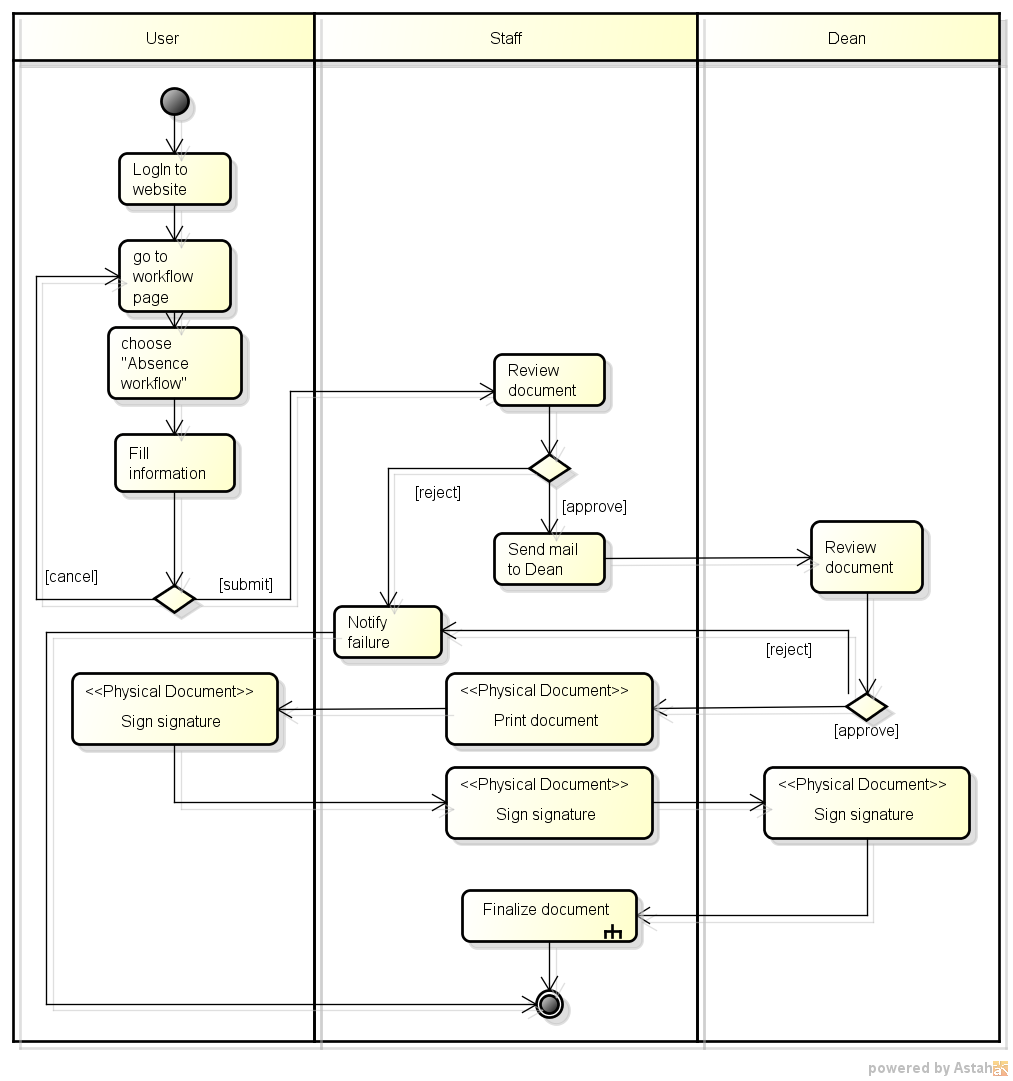
\includegraphics[scale=0.5]{res/Methodology/absence}
\end{figure}

\begin{figure}
	\centering
	\caption{An activity diagram for \enquote{Student internship form}}
	\label{fig:diagram-student-internship}
	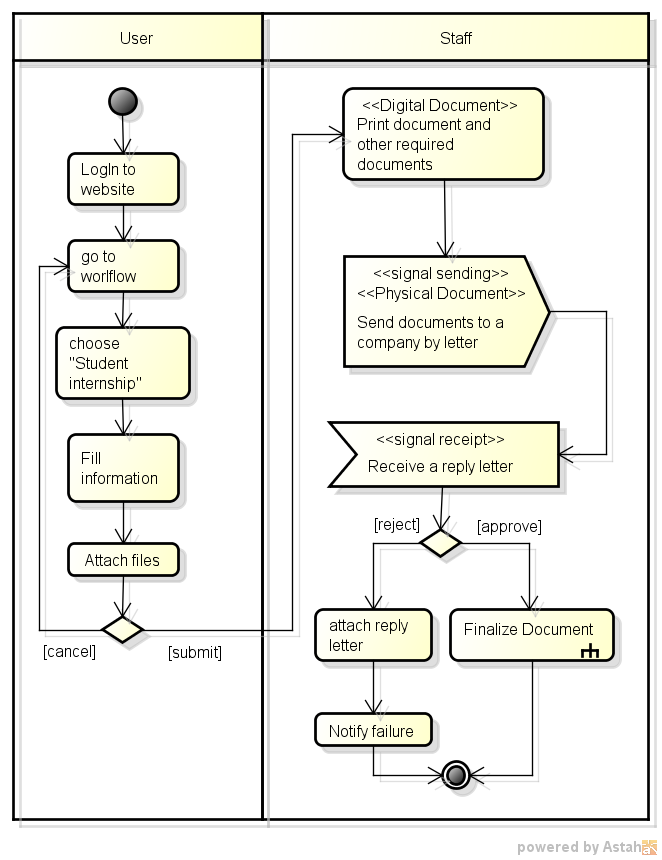
\includegraphics[scale=0.7]{res/Methodology/student_internship}
\end{figure}

\begin{figure}
	\centering
	\caption{An activity diagram for \enquote{Conference outside \gls{kmitl} form}}
	\label{fig:diagram-conference}
	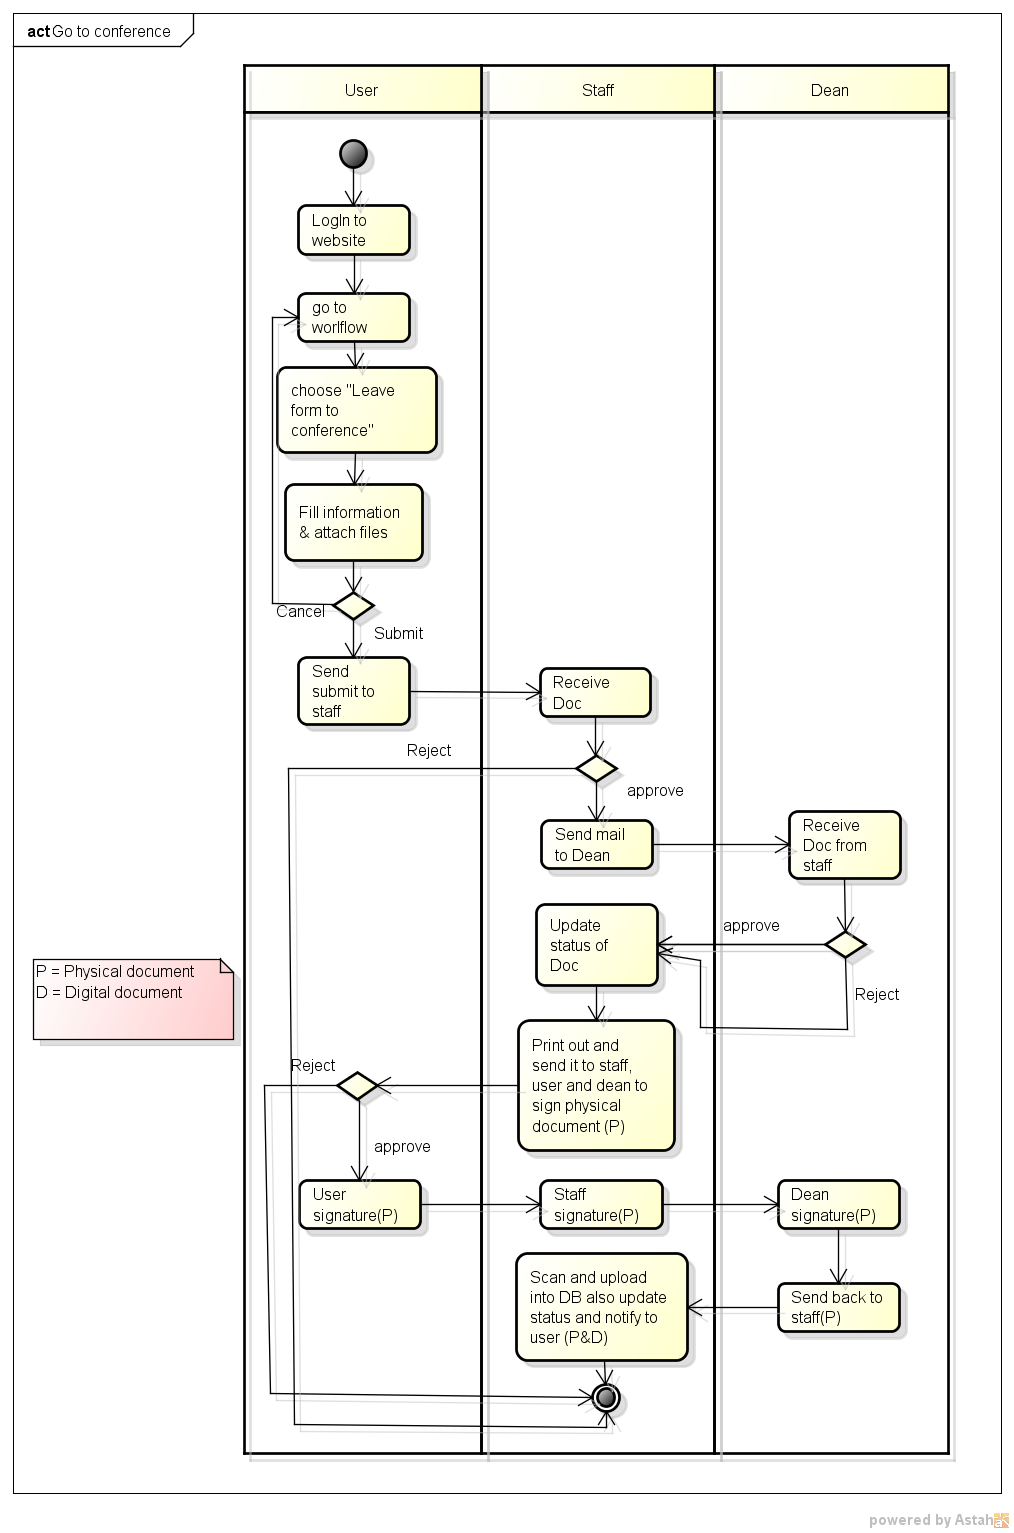
\includegraphics[scale=0.5]{res/Methodology/conference}
\end{figure}

\begin{figure}
	\centering
	\caption{A sub activity diagram of task \enquote{Finalize document}}
	\label{fig:diagram-finalize-document}
	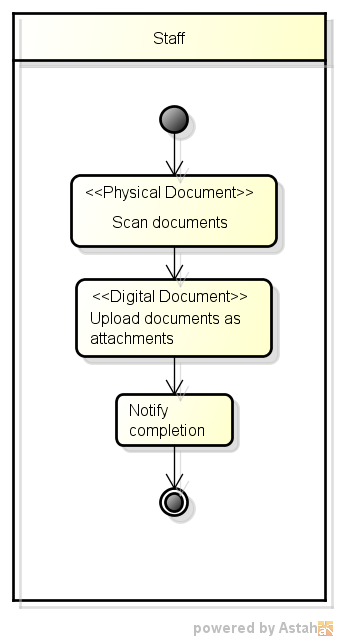
\includegraphics[scale=0.5]{res/Methodology/finalize_document}
\end{figure}

\section{Requirement Summary}
This section summarizes software requirements into itemized lists.
There are two subsections, user requirement and system requirement.

\subsection{User Requirement}
User requirement is a goal or task that specific classes of users must be able to perform with a system, or a desired product attribute \cite{wiegers_2003}.
\begin{enumerate}
	\item 
	User shall be able to includes digital attachment files to the document as it states.
	
	\item
	Staff and dean shall be able to read documents.
	Then perform either the following actions: reject or approve the document.
	
	\item
	Staff shall be able to print out paper documents from digital documents including attachments.
	
	\item
	If any official document requires physical signature(s) as a conclusive evidence, staff shall be able to scan and upload that document as an attachment.
	
	\item
	Any \gls{ic} personnel who have a write-access to official documents shall have read-access to all previous versions of those documents.
	
	\item
	User shall be able to search their documents by the following criteria:
	\subitem A document identification code given by the system.
	\subitem A Form's name.
	\subitem A date when the document is created.
	\subitem A Document's status indicates whether the document is rejected, pending, or completed successfully.
	
	Any mentioned criteria can be mixed together to create more complex search queries.
	
	\item
	\label{notification-method}
	User should be notified when their documents are rejected or completed successfully.
	The notification only happens inside the system.
	Meaning that user require to access the system in order to get notified.
	The system notify user by updating document's status to a new one.
	
	\item
	Staff and dean should be notified when there is a new pending document forwarded to them.
	The notification method is the same as \ref{notification-method}.
\end{enumerate}

\subsection{System Requirement}
System requirement is a top-level requirement for a product that contains multiple subsystems, which could be all software or software and hardware \cite{wiegers_2003}.
\begin{enumerate}
	\item The system shall operate as a web application hosted on a web server so that all users can access it in one place.
	\item The system shall not disclose internal workflow to any user for all associated documents except for an administrator.
	\item The system shall assign an identification code to official documents in the following format: $TTYYYYDDDD$ where
	\subitem $TT$ is the identification code from table \ref{tbl-doc-subtype}.
	\subitem $YYYY$ is the four-digit full Christian year such as 2016 or 2015.
	\subitem $DDDD$ is the four-digit number of the document started at one and increment by one filled with leading zeros.
	\item The system shall contain the REST \gls{api} so that it can communicate with front-end of this system.
	The \gls{api} shall not be publicly available.
	The \gls{api} shall be in URI \enquote{/api/document/\textless interface \textgreater/} where \textless interface \textgreater is the name of the interface.
	URI, input parameter, output, and description are shown in table \ref{tbl:dms-api}.
\end{enumerate}

\begin{table}[h]
	\caption{A list of \gls{api} of this system}
	\label{tbl:dms-api}
	\begin{tabular}{lcL{3.5cm}L{3.5cm}}
		\hline
		URI & Parameter(s) & Return Value (JSON) & Description \\
		\hline
		
		/api/document/read & User ID, Document ID & A document's metadata on a given ID. & Query a document. \\
		
		/api/document/ref & User ID, Document ID & All previous version of the document & Query all previous version of the document on a given ID. \\
		 
		/api/document/attach & User ID, Document ID & Document's attachments & Query all document's attachment files on a given ID. \\
		
		/api/document/attach & User ID & Document's attachments & Query all user's attachment files in all user's documents. \\
		
		/api/document/delete & User ID, Document ID & \gls{http} response & Delete user's document on a given ID.
		The system must not delete other documents owned by a different user. \\
		\hline
	\end{tabular}
\end{table}


\subsection{Quality Attribute}
Quality attribute is a kind of non-functional requirement that describes a service or performance characteristic of a product \cite{wiegers_2003}.
\begin{enumerate}
	\item The system shall encrypt all documents and attachment files.
	\item The system shall use HTTPS communication protocol to exchange data between a web server and a client.
	\item A user interface should have an English localization available.
	\item A user interface should be intuitive enough that user don't have to rely on a user manual.
	Meaning that user doesn't have to go through many processes to achieve their tasks.
	Big buttons and large self-explanatory texts are also preferable.
\end{enumerate}
